\documentclass[twoside]{book}

% Packages required by doxygen
\usepackage{calc}
\usepackage{doxygen}
\usepackage{graphicx}
\usepackage[utf8]{inputenc}
\usepackage{makeidx}
\usepackage{multicol}
\usepackage{multirow}
\usepackage{textcomp}
\usepackage[table]{xcolor}

% Font selection
\usepackage[T1]{fontenc}
\usepackage{mathptmx}
\usepackage[scaled=.90]{helvet}
\usepackage{courier}
\usepackage{amssymb}
\usepackage{sectsty}
\renewcommand{\familydefault}{\sfdefault}
\allsectionsfont{%
  \fontseries{bc}\selectfont%
  \color{darkgray}%
}
\renewcommand{\DoxyLabelFont}{%
  \fontseries{bc}\selectfont%
  \color{darkgray}%
}

% Page & text layout
\usepackage{geometry}
\geometry{%
  a4paper,%
  top=2.5cm,%
  bottom=2.5cm,%
  left=2.5cm,%
  right=2.5cm%
}
\tolerance=750
\hfuzz=15pt
\hbadness=750
\setlength{\emergencystretch}{15pt}
\setlength{\parindent}{0cm}
\setlength{\parskip}{0.2cm}
\makeatletter
\renewcommand{\paragraph}{%
  \@startsection{paragraph}{4}{0ex}{-1.0ex}{1.0ex}{%
    \normalfont\normalsize\bfseries\SS@parafont%
  }%
}
\renewcommand{\subparagraph}{%
  \@startsection{subparagraph}{5}{0ex}{-1.0ex}{1.0ex}{%
    \normalfont\normalsize\bfseries\SS@subparafont%
  }%
}
\makeatother

% Headers & footers
\usepackage{fancyhdr}
\pagestyle{fancyplain}
\fancyhead[LE]{\fancyplain{}{\bfseries\thepage}}
\fancyhead[CE]{\fancyplain{}{}}
\fancyhead[RE]{\fancyplain{}{\bfseries\leftmark}}
\fancyhead[LO]{\fancyplain{}{\bfseries\rightmark}}
\fancyhead[CO]{\fancyplain{}{}}
\fancyhead[RO]{\fancyplain{}{\bfseries\thepage}}
\fancyfoot[LE]{\fancyplain{}{}}
\fancyfoot[CE]{\fancyplain{}{}}
\fancyfoot[RE]{\fancyplain{}{\bfseries\scriptsize Generated on Thu Dec 21 2017 01\-:03\-:45 for Othello by Doxygen }}
\fancyfoot[LO]{\fancyplain{}{\bfseries\scriptsize Generated on Thu Dec 21 2017 01\-:03\-:45 for Othello by Doxygen }}
\fancyfoot[CO]{\fancyplain{}{}}
\fancyfoot[RO]{\fancyplain{}{}}
\renewcommand{\footrulewidth}{0.4pt}
\renewcommand{\chaptermark}[1]{%
  \markboth{#1}{}%
}
\renewcommand{\sectionmark}[1]{%
  \markright{\thesection\ #1}%
}

% Indices & bibliography
\usepackage{natbib}
\usepackage[titles]{tocloft}
\setcounter{tocdepth}{3}
\setcounter{secnumdepth}{5}
\makeindex

% Hyperlinks (required, but should be loaded last)
\usepackage{ifpdf}
\ifpdf
  \usepackage[pdftex,pagebackref=true]{hyperref}
\else
  \usepackage[ps2pdf,pagebackref=true]{hyperref}
\fi
\hypersetup{%
  colorlinks=true,%
  linkcolor=blue,%
  citecolor=blue,%
  unicode%
}

% Custom commands
\newcommand{\clearemptydoublepage}{%
  \newpage{\pagestyle{empty}\cleardoublepage}%
}


%===== C O N T E N T S =====

\begin{document}

% Titlepage & ToC
\hypersetup{pageanchor=false}
\pagenumbering{roman}
\begin{titlepage}
\vspace*{7cm}
\begin{center}%
{\Large Othello }\\
\vspace*{1cm}
{\large Generated by Doxygen 1.8.6}\\
\vspace*{0.5cm}
{\small Thu Dec 21 2017 01:03:45}\\
\end{center}
\end{titlepage}
\clearemptydoublepage
\tableofcontents
\clearemptydoublepage
\pagenumbering{arabic}
\hypersetup{pageanchor=true}

%--- Begin generated contents ---
\chapter{Hierarchical Index}
\section{Class Hierarchy}
This inheritance list is sorted roughly, but not completely, alphabetically\-:\begin{DoxyCompactList}
\item \contentsline{section}{Othello\-Arbiter}{\pageref{classOthelloArbiter}}{}
\item \contentsline{section}{Othello\-Arbiter\-Client}{\pageref{classOthelloArbiterClient}}{}
\item \contentsline{section}{Othello\-Board$<$ N, M $>$}{\pageref{classOthelloBoard}}{}
\item \contentsline{section}{Othello\-Menu}{\pageref{classOthelloMenu}}{}
\item \contentsline{section}{Othello\-Player}{\pageref{classOthelloPlayer}}{}
\begin{DoxyCompactList}
\item \contentsline{section}{Othello\-Player\-C\-E\-S}{\pageref{classOthelloPlayerCES}}{}
\item \contentsline{section}{Othello\-Player\-Human}{\pageref{classOthelloPlayerHuman}}{}
\item \contentsline{section}{Othello\-Player\-L\-O\-M}{\pageref{classOthelloPlayerLOM}}{}
\item \contentsline{section}{Othello\-Player\-Random}{\pageref{classOthelloPlayerRandom}}{}
\item \contentsline{section}{Othello\-Player\-Remote}{\pageref{classOthelloPlayerRemote}}{}
\item \contentsline{section}{Othello\-Player\-Telnet}{\pageref{classOthelloPlayerTelnet}}{}
\end{DoxyCompactList}
\end{DoxyCompactList}

\chapter{Class Index}
\section{Class List}
Here are the classes, structs, unions and interfaces with brief descriptions\-:\begin{DoxyCompactList}
\item\contentsline{section}{\hyperlink{classOthelloArbiter}{Othello\-Arbiter} }{\pageref{classOthelloArbiter}}{}
\item\contentsline{section}{\hyperlink{classOthelloArbiterClient}{Othello\-Arbiter\-Client} }{\pageref{classOthelloArbiterClient}}{}
\item\contentsline{section}{\hyperlink{classOthelloBoard}{Othello\-Board$<$ N, M $>$} }{\pageref{classOthelloBoard}}{}
\item\contentsline{section}{\hyperlink{classOthelloMenu}{Othello\-Menu} }{\pageref{classOthelloMenu}}{}
\item\contentsline{section}{\hyperlink{classOthelloPlayer}{Othello\-Player} }{\pageref{classOthelloPlayer}}{}
\item\contentsline{section}{\hyperlink{classOthelloPlayerCES}{Othello\-Player\-C\-E\-S} }{\pageref{classOthelloPlayerCES}}{}
\item\contentsline{section}{\hyperlink{classOthelloPlayerHuman}{Othello\-Player\-Human} }{\pageref{classOthelloPlayerHuman}}{}
\item\contentsline{section}{\hyperlink{classOthelloPlayerLOM}{Othello\-Player\-L\-O\-M} }{\pageref{classOthelloPlayerLOM}}{}
\item\contentsline{section}{\hyperlink{classOthelloPlayerRandom}{Othello\-Player\-Random} }{\pageref{classOthelloPlayerRandom}}{}
\item\contentsline{section}{\hyperlink{classOthelloPlayerRemote}{Othello\-Player\-Remote} }{\pageref{classOthelloPlayerRemote}}{}
\item\contentsline{section}{\hyperlink{classOthelloPlayerTelnet}{Othello\-Player\-Telnet} }{\pageref{classOthelloPlayerTelnet}}{}
\end{DoxyCompactList}

\chapter{Class Documentation}
\hypertarget{classOthelloArbiter}{\section{Othello\-Arbiter Class Reference}
\label{classOthelloArbiter}\index{Othello\-Arbiter@{Othello\-Arbiter}}
}
\subsection*{Public Member Functions}
\begin{DoxyCompactItemize}
\item 
\hypertarget{classOthelloArbiter_a9262380107a3219aeb8b332a88fafcbf}{void {\bfseries add\-Player} (\hyperlink{classOthelloPlayer}{Othello\-Player} $\ast$const player)}\label{classOthelloArbiter_a9262380107a3219aeb8b332a88fafcbf}

\item 
\hypertarget{classOthelloArbiter_ae749a8f06d8037f8c193bd87a18611da}{unsigned char {\bfseries play\-Othello} ()}\label{classOthelloArbiter_ae749a8f06d8037f8c193bd87a18611da}

\item 
\hypertarget{classOthelloArbiter_a3d2341554a6be0ad0ecb46fc3aa35068}{void {\bfseries set\-Verbosity} (int verbosity)}\label{classOthelloArbiter_a3d2341554a6be0ad0ecb46fc3aa35068}

\item 
\hypertarget{classOthelloArbiter_a7bb8ba1e1db1b3cfc7033b88fb32f219}{{\bfseries Othello\-Arbiter} (int sockd)}\label{classOthelloArbiter_a7bb8ba1e1db1b3cfc7033b88fb32f219}

\end{DoxyCompactItemize}


The documentation for this class was generated from the following files\-:\begin{DoxyCompactItemize}
\item 
/home/travis/build/pastika/\-Othello/othello\-Arbiter.\-h\item 
/home/travis/build/pastika/\-Othello/othello\-Arbiter.\-cpp\end{DoxyCompactItemize}

\hypertarget{classOthelloArbiterClient}{\section{Othello\-Arbiter\-Client Class Reference}
\label{classOthelloArbiterClient}\index{Othello\-Arbiter\-Client@{Othello\-Arbiter\-Client}}
}
\subsection*{Public Member Functions}
\begin{DoxyCompactItemize}
\item 
\hypertarget{classOthelloArbiterClient_afbaee18450509edf7a5d131d62f2fbe9}{{\bfseries Othello\-Arbiter\-Client} (int sockd)}\label{classOthelloArbiterClient_afbaee18450509edf7a5d131d62f2fbe9}

\item 
\hypertarget{classOthelloArbiterClient_a9020db71b40c949e9ea2b6edfccb0df9}{void {\bfseries set\-Player} (\hyperlink{classOthelloPlayer}{Othello\-Player} $\ast$player)}\label{classOthelloArbiterClient_a9020db71b40c949e9ea2b6edfccb0df9}

\item 
\hypertarget{classOthelloArbiterClient_ad14af76840bc25e19396fbad7a713333}{void {\bfseries set\-Verbosity} (int verbosity)}\label{classOthelloArbiterClient_ad14af76840bc25e19396fbad7a713333}

\item 
\hypertarget{classOthelloArbiterClient_a710bc44f7d82eff7937071dbeab1ff6a}{void {\bfseries begin\-Arbitration} ()}\label{classOthelloArbiterClient_a710bc44f7d82eff7937071dbeab1ff6a}

\end{DoxyCompactItemize}


The documentation for this class was generated from the following files\-:\begin{DoxyCompactItemize}
\item 
/home/travis/build/pastika/\-Othello/othello\-Arbiter\-Client.\-h\item 
/home/travis/build/pastika/\-Othello/othello\-Arbiter\-Client.\-cpp\end{DoxyCompactItemize}

\hypertarget{classOthelloBoard}{\section{Othello\-Board$<$ N, M $>$ Class Template Reference}
\label{classOthelloBoard}\index{Othello\-Board$<$ N, M $>$@{Othello\-Board$<$ N, M $>$}}
}


{\ttfamily \#include $<$othello\-Board.\-h$>$}

\subsection*{Public Member Functions}
\begin{DoxyCompactItemize}
\item 
\hyperlink{classOthelloBoard_a3f996705018ff9d27657bc0b724e857f}{Othello\-Board} ()
\item 
const std\-::string \hyperlink{classOthelloBoard_a91b476e5d89605400e93eab7f2f3ca2d}{package\-Board} () const 
\item 
bool \hyperlink{classOthelloBoard_ae2ac8bc8fd191a029207fcd5ad096d92}{construct\-Board} (const std\-::string board\-Package)
\item 
unsigned char \hyperlink{classOthelloBoard_a2303029a0e36c94dcc12903592287e3a}{winner} () const 
\item 
int \hyperlink{classOthelloBoard_a876a2168b743b1a36d58f8191bd2bda0}{avaliable\-Moves} (const unsigned char player)
\item 
bool \hyperlink{classOthelloBoard_a9d50536c87a0e73882d845815bf72b65}{play} (const unsigned char player, const int x, const int y)
\item 
void \hyperlink{classOthelloBoard_aeb67c1d90f64fee5c1c63fbfe4330a11}{print} () const 
\item 
void \hyperlink{classOthelloBoard_a76077193286df75737e0ce23e83bb70c}{construct\-Display\-String} (std\-::stringstream \&ssdstr) const 
\item 
char \hyperlink{classOthelloBoard_ac33b6f65bc0e95efb82519ea36b07c1e}{player\-To\-Char} (const unsigned char player) const 
\item 
const \hyperlink{classOthelloBoard}{Othello\-Board}$<$ 8, 8 $>$ \& \hyperlink{classOthelloBoard_abb88de115c183847aa91a93176404783}{get\-State} () const 
\item 
const std\-::set$<$ std\-::pair$<$ int, \\*
int $>$ $>$ \& \hyperlink{classOthelloBoard_a24c36f4b8d92934aacd63ddfff8a8941}{get\-Valid\-Plays} () const 
\item 
const unsigned char \hyperlink{classOthelloBoard_a3b1d8204a1f096cd818431621453f54d}{get\-Last\-Player} () const 
\end{DoxyCompactItemize}
\subsection*{Static Public Member Functions}
\begin{DoxyCompactItemize}
\item 
static const char $\ast$ \hyperlink{classOthelloBoard_af2812a9e104285af5147e05306ce528f}{player\-To\-Char\-And\-Color} (const unsigned char player)
\end{DoxyCompactItemize}


\subsection{Detailed Description}
\subsubsection*{template$<$const int N, const int M$>$class Othello\-Board$<$ N, M $>$}

\hyperlink{classOthelloBoard}{Othello\-Board} holds an othello board of arbitrary size N by M along with the basic play mechanics of the game. 

\subsection{Constructor \& Destructor Documentation}
\hypertarget{classOthelloBoard_a3f996705018ff9d27657bc0b724e857f}{\index{Othello\-Board@{Othello\-Board}!Othello\-Board@{Othello\-Board}}
\index{Othello\-Board@{Othello\-Board}!OthelloBoard@{Othello\-Board}}
\subsubsection[{Othello\-Board}]{\setlength{\rightskip}{0pt plus 5cm}template$<$const int N, const int M$>$ {\bf Othello\-Board}$<$ N, M $>$\-::{\bf Othello\-Board} (
\begin{DoxyParamCaption}
{}
\end{DoxyParamCaption}
)\hspace{0.3cm}{\ttfamily [inline]}}}\label{classOthelloBoard_a3f996705018ff9d27657bc0b724e857f}
Constructs an empty othello board ready for play. 

\subsection{Member Function Documentation}
\hypertarget{classOthelloBoard_a876a2168b743b1a36d58f8191bd2bda0}{\index{Othello\-Board@{Othello\-Board}!avaliable\-Moves@{avaliable\-Moves}}
\index{avaliable\-Moves@{avaliable\-Moves}!OthelloBoard@{Othello\-Board}}
\subsubsection[{avaliable\-Moves}]{\setlength{\rightskip}{0pt plus 5cm}template$<$const int N, const int M$>$ int {\bf Othello\-Board}$<$ N, M $>$\-::avaliable\-Moves (
\begin{DoxyParamCaption}
\item[{const unsigned char}]{player}
\end{DoxyParamCaption}
)\hspace{0.3cm}{\ttfamily [inline]}}}\label{classOthelloBoard_a876a2168b743b1a36d58f8191bd2bda0}
Calculates the list of legal moves for the player specified 
\begin{DoxyParams}{Parameters}
{\em player} & Player to calculate the legal moves for \\
\hline
\end{DoxyParams}
\begin{DoxyReturn}{Returns}
The number of legal moves for player 
\end{DoxyReturn}
\hypertarget{classOthelloBoard_ae2ac8bc8fd191a029207fcd5ad096d92}{\index{Othello\-Board@{Othello\-Board}!construct\-Board@{construct\-Board}}
\index{construct\-Board@{construct\-Board}!OthelloBoard@{Othello\-Board}}
\subsubsection[{construct\-Board}]{\setlength{\rightskip}{0pt plus 5cm}template$<$const int N, const int M$>$ bool {\bf Othello\-Board}$<$ N, M $>$\-::construct\-Board (
\begin{DoxyParamCaption}
\item[{const std\-::string}]{board\-Package}
\end{DoxyParamCaption}
)\hspace{0.3cm}{\ttfamily [inline]}}}\label{classOthelloBoard_ae2ac8bc8fd191a029207fcd5ad096d92}
Reconstructs an othello board state from a packaged board string 
\begin{DoxyParams}{Parameters}
{\em board\-Package} & string produced by package\-Board to decode \\
\hline
\end{DoxyParams}
\begin{DoxyReturn}{Returns}
returns true if the string is successfully parsed, otherwise false 
\end{DoxyReturn}
\hypertarget{classOthelloBoard_a76077193286df75737e0ce23e83bb70c}{\index{Othello\-Board@{Othello\-Board}!construct\-Display\-String@{construct\-Display\-String}}
\index{construct\-Display\-String@{construct\-Display\-String}!OthelloBoard@{Othello\-Board}}
\subsubsection[{construct\-Display\-String}]{\setlength{\rightskip}{0pt plus 5cm}template$<$const int N, const int M$>$ void {\bf Othello\-Board}$<$ N, M $>$\-::construct\-Display\-String (
\begin{DoxyParamCaption}
\item[{std\-::stringstream \&}]{ssdstr}
\end{DoxyParamCaption}
) const\hspace{0.3cm}{\ttfamily [inline]}}}\label{classOthelloBoard_a76077193286df75737e0ce23e83bb70c}
Helper function to construct the current stringstream for the current board state 
\begin{DoxyParams}{Parameters}
{\em ssdstr} & Stringstream object to fill with the current board state \\
\hline
\end{DoxyParams}
\hypertarget{classOthelloBoard_a3b1d8204a1f096cd818431621453f54d}{\index{Othello\-Board@{Othello\-Board}!get\-Last\-Player@{get\-Last\-Player}}
\index{get\-Last\-Player@{get\-Last\-Player}!OthelloBoard@{Othello\-Board}}
\subsubsection[{get\-Last\-Player}]{\setlength{\rightskip}{0pt plus 5cm}template$<$const int N, const int M$>$ const unsigned char {\bf Othello\-Board}$<$ N, M $>$\-::get\-Last\-Player (
\begin{DoxyParamCaption}
{}
\end{DoxyParamCaption}
) const\hspace{0.3cm}{\ttfamily [inline]}}}\label{classOthelloBoard_a3b1d8204a1f096cd818431621453f54d}
The last player to go before the current player \begin{DoxyReturn}{Returns}
The last player to go before the current player 
\end{DoxyReturn}
\hypertarget{classOthelloBoard_abb88de115c183847aa91a93176404783}{\index{Othello\-Board@{Othello\-Board}!get\-State@{get\-State}}
\index{get\-State@{get\-State}!OthelloBoard@{Othello\-Board}}
\subsubsection[{get\-State}]{\setlength{\rightskip}{0pt plus 5cm}template$<$const int N, const int M$>$ const {\bf Othello\-Board}$<$8, 8$>$\& {\bf Othello\-Board}$<$ N, M $>$\-::get\-State (
\begin{DoxyParamCaption}
{}
\end{DoxyParamCaption}
) const\hspace{0.3cm}{\ttfamily [inline]}}}\label{classOthelloBoard_abb88de115c183847aa91a93176404783}
Returns the current state of the \hyperlink{classOthelloBoard}{Othello\-Board} object \begin{DoxyReturn}{Returns}
The current state of the \hyperlink{classOthelloBoard}{Othello\-Board} object 
\end{DoxyReturn}
\hypertarget{classOthelloBoard_a24c36f4b8d92934aacd63ddfff8a8941}{\index{Othello\-Board@{Othello\-Board}!get\-Valid\-Plays@{get\-Valid\-Plays}}
\index{get\-Valid\-Plays@{get\-Valid\-Plays}!OthelloBoard@{Othello\-Board}}
\subsubsection[{get\-Valid\-Plays}]{\setlength{\rightskip}{0pt plus 5cm}template$<$const int N, const int M$>$ const std\-::set$<$std\-::pair$<$int, int$>$ $>$\& {\bf Othello\-Board}$<$ N, M $>$\-::get\-Valid\-Plays (
\begin{DoxyParamCaption}
{}
\end{DoxyParamCaption}
) const\hspace{0.3cm}{\ttfamily [inline]}}}\label{classOthelloBoard_a24c36f4b8d92934aacd63ddfff8a8941}
Getter to return the list of valid plays for the current player \begin{DoxyReturn}{Returns}
The set of valid plays for the current player 
\end{DoxyReturn}
\hypertarget{classOthelloBoard_a91b476e5d89605400e93eab7f2f3ca2d}{\index{Othello\-Board@{Othello\-Board}!package\-Board@{package\-Board}}
\index{package\-Board@{package\-Board}!OthelloBoard@{Othello\-Board}}
\subsubsection[{package\-Board}]{\setlength{\rightskip}{0pt plus 5cm}template$<$const int N, const int M$>$ const std\-::string {\bf Othello\-Board}$<$ N, M $>$\-::package\-Board (
\begin{DoxyParamCaption}
{}
\end{DoxyParamCaption}
) const\hspace{0.3cm}{\ttfamily [inline]}}}\label{classOthelloBoard_a91b476e5d89605400e93eab7f2f3ca2d}
Translates the internal board array into a single non-\/human readable string which is intended for transmission via network to another client. \begin{DoxyReturn}{Returns}
Packaged string containing all the information in the internal board array 
\end{DoxyReturn}
\hypertarget{classOthelloBoard_a9d50536c87a0e73882d845815bf72b65}{\index{Othello\-Board@{Othello\-Board}!play@{play}}
\index{play@{play}!OthelloBoard@{Othello\-Board}}
\subsubsection[{play}]{\setlength{\rightskip}{0pt plus 5cm}template$<$const int N, const int M$>$ bool {\bf Othello\-Board}$<$ N, M $>$\-::play (
\begin{DoxyParamCaption}
\item[{const unsigned char}]{player, }
\item[{const int}]{x, }
\item[{const int}]{y}
\end{DoxyParamCaption}
)\hspace{0.3cm}{\ttfamily [inline]}}}\label{classOthelloBoard_a9d50536c87a0e73882d845815bf72b65}
Place a piece on the board for the specified player. 
\begin{DoxyParams}{Parameters}
{\em player} & the player who is placing the piece \\
\hline
{\em x} & the x position to place the piece \\
\hline
{\em y} & the y position to place the piece \\
\hline
\end{DoxyParams}
\begin{DoxyReturn}{Returns}
If the move was a legal move returns true, otherwise the piece is not placed and the function returns false 
\end{DoxyReturn}
\hypertarget{classOthelloBoard_ac33b6f65bc0e95efb82519ea36b07c1e}{\index{Othello\-Board@{Othello\-Board}!player\-To\-Char@{player\-To\-Char}}
\index{player\-To\-Char@{player\-To\-Char}!OthelloBoard@{Othello\-Board}}
\subsubsection[{player\-To\-Char}]{\setlength{\rightskip}{0pt plus 5cm}template$<$const int N, const int M$>$ char {\bf Othello\-Board}$<$ N, M $>$\-::player\-To\-Char (
\begin{DoxyParamCaption}
\item[{const unsigned char}]{player}
\end{DoxyParamCaption}
) const\hspace{0.3cm}{\ttfamily [inline]}}}\label{classOthelloBoard_ac33b6f65bc0e95efb82519ea36b07c1e}
Helper function to convert the current player number into the approperiate display symbol on the screen. 
\begin{DoxyParams}{Parameters}
{\em player} & The player to return the symbol for \\
\hline
\end{DoxyParams}
\begin{DoxyReturn}{Returns}
The symbol corropsonding to player 
\end{DoxyReturn}
\hypertarget{classOthelloBoard_af2812a9e104285af5147e05306ce528f}{\index{Othello\-Board@{Othello\-Board}!player\-To\-Char\-And\-Color@{player\-To\-Char\-And\-Color}}
\index{player\-To\-Char\-And\-Color@{player\-To\-Char\-And\-Color}!OthelloBoard@{Othello\-Board}}
\subsubsection[{player\-To\-Char\-And\-Color}]{\setlength{\rightskip}{0pt plus 5cm}template$<$const int N, const int M$>$ static const char$\ast$ {\bf Othello\-Board}$<$ N, M $>$\-::player\-To\-Char\-And\-Color (
\begin{DoxyParamCaption}
\item[{const unsigned char}]{player}
\end{DoxyParamCaption}
)\hspace{0.3cm}{\ttfamily [inline]}, {\ttfamily [static]}}}\label{classOthelloBoard_af2812a9e104285af5147e05306ce528f}
Helper function to convert the current player number into the approperiate display symbol on the screen with color. 
\begin{DoxyParams}{Parameters}
{\em player} & The player to return the symbol for \\
\hline
\end{DoxyParams}
\begin{DoxyReturn}{Returns}
The symbol corropsonding to player 
\end{DoxyReturn}
\hypertarget{classOthelloBoard_aeb67c1d90f64fee5c1c63fbfe4330a11}{\index{Othello\-Board@{Othello\-Board}!print@{print}}
\index{print@{print}!OthelloBoard@{Othello\-Board}}
\subsubsection[{print}]{\setlength{\rightskip}{0pt plus 5cm}template$<$const int N, const int M$>$ void {\bf Othello\-Board}$<$ N, M $>$\-::print (
\begin{DoxyParamCaption}
{}
\end{DoxyParamCaption}
) const\hspace{0.3cm}{\ttfamily [inline]}}}\label{classOthelloBoard_aeb67c1d90f64fee5c1c63fbfe4330a11}
Print the current board state to the screen. \hypertarget{classOthelloBoard_a2303029a0e36c94dcc12903592287e3a}{\index{Othello\-Board@{Othello\-Board}!winner@{winner}}
\index{winner@{winner}!OthelloBoard@{Othello\-Board}}
\subsubsection[{winner}]{\setlength{\rightskip}{0pt plus 5cm}template$<$const int N, const int M$>$ unsigned char {\bf Othello\-Board}$<$ N, M $>$\-::winner (
\begin{DoxyParamCaption}
{}
\end{DoxyParamCaption}
) const\hspace{0.3cm}{\ttfamily [inline]}}}\label{classOthelloBoard_a2303029a0e36c94dcc12903592287e3a}
Determine which player currently is willing the game. I.\-e. who has the most pieces of the board. \begin{DoxyReturn}{Returns}
returns the player who currently has the most pieces of the baord 
\end{DoxyReturn}


The documentation for this class was generated from the following file\-:\begin{DoxyCompactItemize}
\item 
/home/travis/build/pastika/\-Othello/othello\-Board.\-h\end{DoxyCompactItemize}

\hypertarget{classOthelloMenu}{\section{Othello\-Menu Class Reference}
\label{classOthelloMenu}\index{Othello\-Menu@{Othello\-Menu}}
}
\subsection*{Public Types}
\begin{DoxyCompactItemize}
\item 
enum {\bfseries O\-T\-H\-E\-L\-L\-O\-S\-T\-A\-T\-E} \{ \\*
{\bfseries O\-S\-\_\-\-E\-X\-I\-T}, 
{\bfseries O\-S\-\_\-\-S\-T\-A\-R\-T\-M\-E\-N\-U}, 
{\bfseries O\-S\-\_\-\-S\-E\-T\-P\-L\-A\-Y\-E\-R\-S\-L\-O\-T}, 
{\bfseries O\-S\-\_\-\-S\-E\-T\-O\-P\-P\-O\-N\-E\-N\-T}, 
\\*
{\bfseries O\-S\-\_\-\-P\-L\-A\-Y}
 \}
\end{DoxyCompactItemize}
\subsection*{Public Member Functions}
\begin{DoxyCompactItemize}
\item 
\hypertarget{classOthelloMenu_a6495e2635b5eace0d299d64ec24af66f}{{\bfseries Othello\-Menu} (int sockd)}\label{classOthelloMenu_a6495e2635b5eace0d299d64ec24af66f}

\item 
\hypertarget{classOthelloMenu_a28538903d5b5978a77d9269da29d7657}{void {\bfseries set\-Verbosity} (const int verbosity)}\label{classOthelloMenu_a28538903d5b5978a77d9269da29d7657}

\item 
\hypertarget{classOthelloMenu_a2f3bb0dfd1a33ca5d24392514f6deae2}{int {\bfseries start\-Menu} ()}\label{classOthelloMenu_a2f3bb0dfd1a33ca5d24392514f6deae2}

\item 
\hypertarget{classOthelloMenu_a26ce1dde06b0eb79ce5c167046002e20}{\hyperlink{classOthelloPlayer}{Othello\-Player} $\ast$ {\bfseries get\-Player1} ()}\label{classOthelloMenu_a26ce1dde06b0eb79ce5c167046002e20}

\item 
\hypertarget{classOthelloMenu_a95ff349f9abd80ef527a915fc2e10042}{\hyperlink{classOthelloPlayer}{Othello\-Player} $\ast$ {\bfseries get\-Player2} ()}\label{classOthelloMenu_a95ff349f9abd80ef527a915fc2e10042}

\end{DoxyCompactItemize}


The documentation for this class was generated from the following file\-:\begin{DoxyCompactItemize}
\item 
/home/travis/build/pastika/\-Othello/othello\-Menu.\-h\end{DoxyCompactItemize}

\hypertarget{classOthelloPlayer}{\section{Othello\-Player Class Reference}
\label{classOthelloPlayer}\index{Othello\-Player@{Othello\-Player}}
}


{\ttfamily \#include $<$othello\-Player.\-h$>$}

Inheritance diagram for Othello\-Player\-:\begin{figure}[H]
\begin{center}
\leavevmode
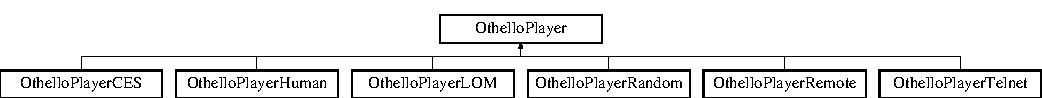
\includegraphics[height=1.314554cm]{classOthelloPlayer}
\end{center}
\end{figure}
\subsection*{Public Member Functions}
\begin{DoxyCompactItemize}
\item 
void \hyperlink{classOthelloPlayer_a9aa0f48e9cb6c1e7c9037850423f2915}{operator()} (const \hyperlink{classOthelloBoard}{Othello\-Board}$<$ 8, 8 $>$ \&board, int \&x, int \&y)
\item 
void \hyperlink{classOthelloPlayer_a856fb93347be5480c9db179bb912c694}{set\-Player} (const unsigned char player)
\item 
virtual void \hyperlink{classOthelloPlayer_a278b0f93b676c302f914a3dac85d5adf}{winner} (const unsigned char winner, const \hyperlink{classOthelloBoard}{Othello\-Board}$<$ 8, 8 $>$ \&board)
\end{DoxyCompactItemize}
\subsection*{Protected Attributes}
\begin{DoxyCompactItemize}
\item 
\hypertarget{classOthelloPlayer_a19f59ab327765eac668851590e7d51f3}{unsigned char \hyperlink{classOthelloPlayer_a19f59ab327765eac668851590e7d51f3}{player\-\_\-}}\label{classOthelloPlayer_a19f59ab327765eac668851590e7d51f3}

\begin{DoxyCompactList}\small\item\em Internal variable to track which player this in the game. \end{DoxyCompactList}\end{DoxyCompactItemize}


\subsection{Detailed Description}
Base class to define an othello player. 

\subsection{Member Function Documentation}
\hypertarget{classOthelloPlayer_a9aa0f48e9cb6c1e7c9037850423f2915}{\index{Othello\-Player@{Othello\-Player}!operator()@{operator()}}
\index{operator()@{operator()}!OthelloPlayer@{Othello\-Player}}
\subsubsection[{operator()}]{\setlength{\rightskip}{0pt plus 5cm}void Othello\-Player\-::operator() (
\begin{DoxyParamCaption}
\item[{const {\bf Othello\-Board}$<$ 8, 8 $>$ \&}]{board, }
\item[{int \&}]{x, }
\item[{int \&}]{y}
\end{DoxyParamCaption}
)\hspace{0.3cm}{\ttfamily [inline]}}}\label{classOthelloPlayer_a9aa0f48e9cb6c1e7c9037850423f2915}
External interface to the return\-Play function. \hypertarget{classOthelloPlayer_a856fb93347be5480c9db179bb912c694}{\index{Othello\-Player@{Othello\-Player}!set\-Player@{set\-Player}}
\index{set\-Player@{set\-Player}!OthelloPlayer@{Othello\-Player}}
\subsubsection[{set\-Player}]{\setlength{\rightskip}{0pt plus 5cm}void Othello\-Player\-::set\-Player (
\begin{DoxyParamCaption}
\item[{const unsigned char}]{player}
\end{DoxyParamCaption}
)\hspace{0.3cm}{\ttfamily [inline]}}}\label{classOthelloPlayer_a856fb93347be5480c9db179bb912c694}
Set which player position in the game this \hyperlink{classOthelloPlayer}{Othello\-Player} will be (1 or 2 for a traditional game) 
\begin{DoxyParams}{Parameters}
{\em The} & assigned player position \\
\hline
\end{DoxyParams}
\hypertarget{classOthelloPlayer_a278b0f93b676c302f914a3dac85d5adf}{\index{Othello\-Player@{Othello\-Player}!winner@{winner}}
\index{winner@{winner}!OthelloPlayer@{Othello\-Player}}
\subsubsection[{winner}]{\setlength{\rightskip}{0pt plus 5cm}virtual void Othello\-Player\-::winner (
\begin{DoxyParamCaption}
\item[{const unsigned char}]{winner, }
\item[{const {\bf Othello\-Board}$<$ 8, 8 $>$ \&}]{board}
\end{DoxyParamCaption}
)\hspace{0.3cm}{\ttfamily [inline]}, {\ttfamily [virtual]}}}\label{classOthelloPlayer_a278b0f93b676c302f914a3dac85d5adf}
This function is used to inform the \hyperlink{classOthelloPlayer}{Othello\-Player} which of the players won the game and provide the final board state. It is optional to redefine this method. The player may choose to ignore this information, in which case the default definition is sufficient. 
\begin{DoxyParams}{Parameters}
{\em winner} & The player position of the winning player \\
\hline
{\em The} & board state at the end of the game \\
\hline
\end{DoxyParams}


Reimplemented in \hyperlink{classOthelloPlayerTelnet_a2903532fbbc2de163b4bf3c14e214dfe}{Othello\-Player\-Telnet}, and \hyperlink{classOthelloPlayerRemote_a6d7f6c0544aa6a6eb219e69d6c6d2e41}{Othello\-Player\-Remote}.



The documentation for this class was generated from the following file\-:\begin{DoxyCompactItemize}
\item 
/home/travis/build/pastika/\-Othello/othello\-Player.\-h\end{DoxyCompactItemize}

\hypertarget{classOthelloPlayerCES}{\section{Othello\-Player\-C\-E\-S Class Reference}
\label{classOthelloPlayerCES}\index{Othello\-Player\-C\-E\-S@{Othello\-Player\-C\-E\-S}}
}
Inheritance diagram for Othello\-Player\-C\-E\-S\-:\begin{figure}[H]
\begin{center}
\leavevmode
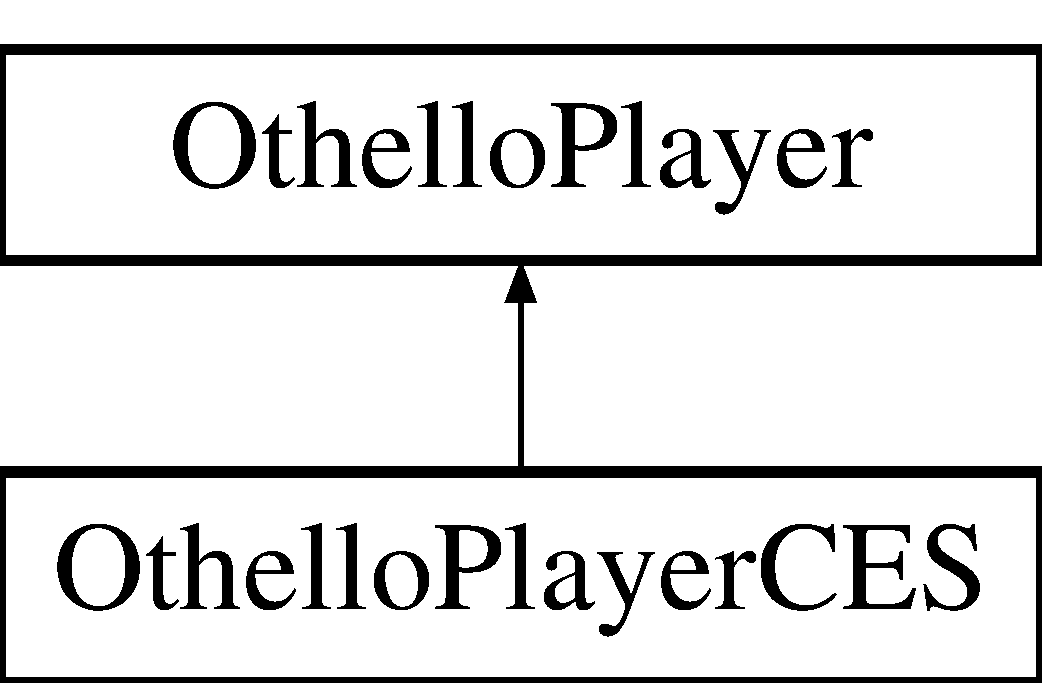
\includegraphics[height=2.000000cm]{classOthelloPlayerCES}
\end{center}
\end{figure}
\subsection*{Additional Inherited Members}


The documentation for this class was generated from the following files\-:\begin{DoxyCompactItemize}
\item 
/home/travis/build/pastika/\-Othello/othello\-Player\-C\-E\-S.\-h\item 
/home/travis/build/pastika/\-Othello/othello\-Player\-C\-E\-S.\-cpp\end{DoxyCompactItemize}

\hypertarget{classOthelloPlayerHuman}{\section{Othello\-Player\-Human Class Reference}
\label{classOthelloPlayerHuman}\index{Othello\-Player\-Human@{Othello\-Player\-Human}}
}
Inheritance diagram for Othello\-Player\-Human\-:\begin{figure}[H]
\begin{center}
\leavevmode
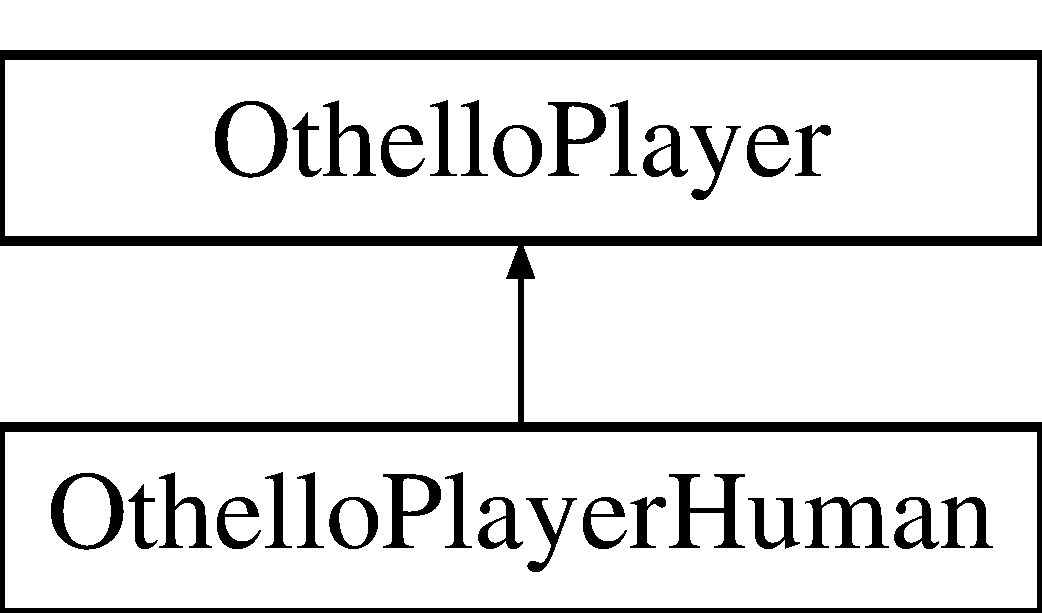
\includegraphics[height=2.000000cm]{classOthelloPlayerHuman}
\end{center}
\end{figure}
\subsection*{Additional Inherited Members}


The documentation for this class was generated from the following file\-:\begin{DoxyCompactItemize}
\item 
/home/travis/build/pastika/\-Othello/othello\-Player\-Human.\-h\end{DoxyCompactItemize}

\hypertarget{classOthelloPlayerLOM}{\section{Othello\-Player\-L\-O\-M Class Reference}
\label{classOthelloPlayerLOM}\index{Othello\-Player\-L\-O\-M@{Othello\-Player\-L\-O\-M}}
}
Inheritance diagram for Othello\-Player\-L\-O\-M\-:\begin{figure}[H]
\begin{center}
\leavevmode
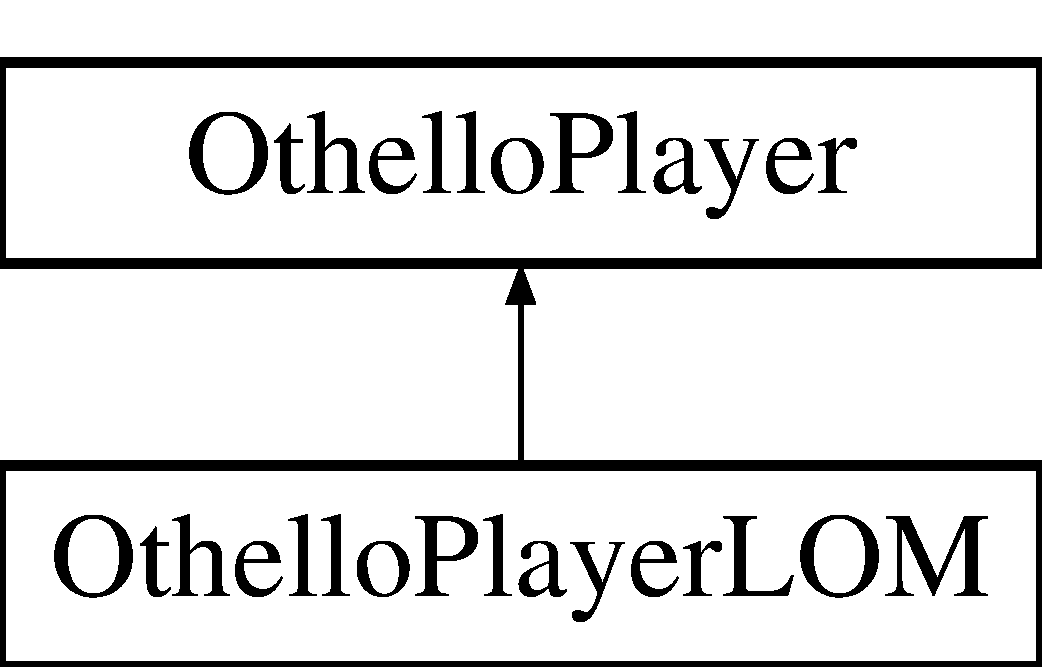
\includegraphics[height=2.000000cm]{classOthelloPlayerLOM}
\end{center}
\end{figure}
\subsection*{Additional Inherited Members}


The documentation for this class was generated from the following files\-:\begin{DoxyCompactItemize}
\item 
/home/travis/build/pastika/\-Othello/othello\-Player\-L\-O\-M.\-h\item 
/home/travis/build/pastika/\-Othello/othello\-Player\-L\-O\-M.\-cpp\end{DoxyCompactItemize}

\hypertarget{classOthelloPlayerRandom}{\section{Othello\-Player\-Random Class Reference}
\label{classOthelloPlayerRandom}\index{Othello\-Player\-Random@{Othello\-Player\-Random}}
}
Inheritance diagram for Othello\-Player\-Random\-:\begin{figure}[H]
\begin{center}
\leavevmode
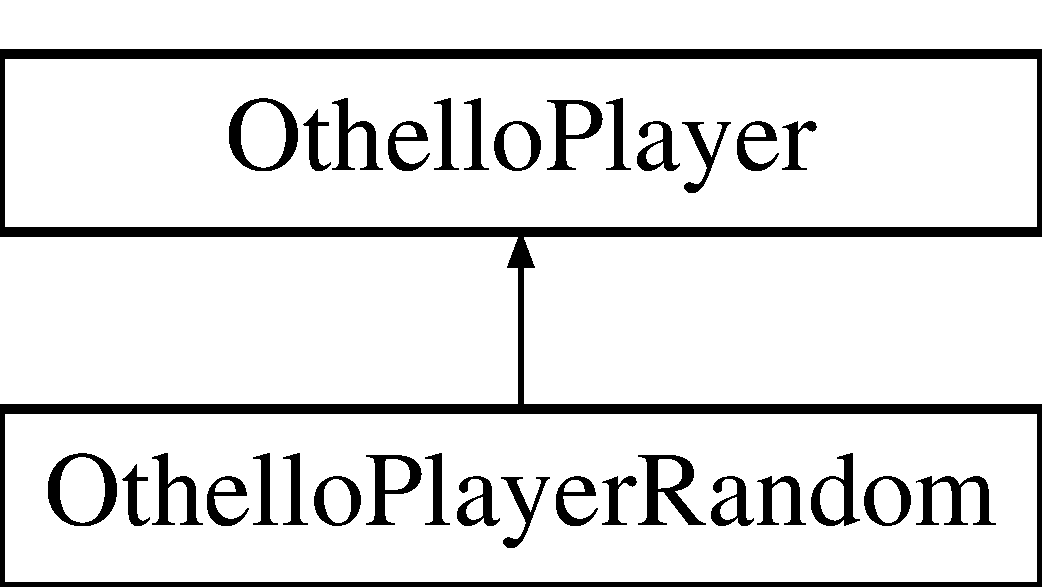
\includegraphics[height=2.000000cm]{classOthelloPlayerRandom}
\end{center}
\end{figure}
\subsection*{Public Member Functions}
\begin{DoxyCompactItemize}
\item 
\hypertarget{classOthelloPlayerRandom_ab997f756b9de745208e3e540c36caf25}{{\bfseries Othello\-Player\-Random} (int seed=12321)}\label{classOthelloPlayerRandom_ab997f756b9de745208e3e540c36caf25}

\end{DoxyCompactItemize}
\subsection*{Additional Inherited Members}


The documentation for this class was generated from the following files\-:\begin{DoxyCompactItemize}
\item 
/home/travis/build/pastika/\-Othello/othello\-Player\-Random.\-h\item 
/home/travis/build/pastika/\-Othello/othello\-Player\-Random.\-cpp\end{DoxyCompactItemize}

\hypertarget{classOthelloPlayerRemote}{\section{Othello\-Player\-Remote Class Reference}
\label{classOthelloPlayerRemote}\index{Othello\-Player\-Remote@{Othello\-Player\-Remote}}
}
Inheritance diagram for Othello\-Player\-Remote\-:\begin{figure}[H]
\begin{center}
\leavevmode
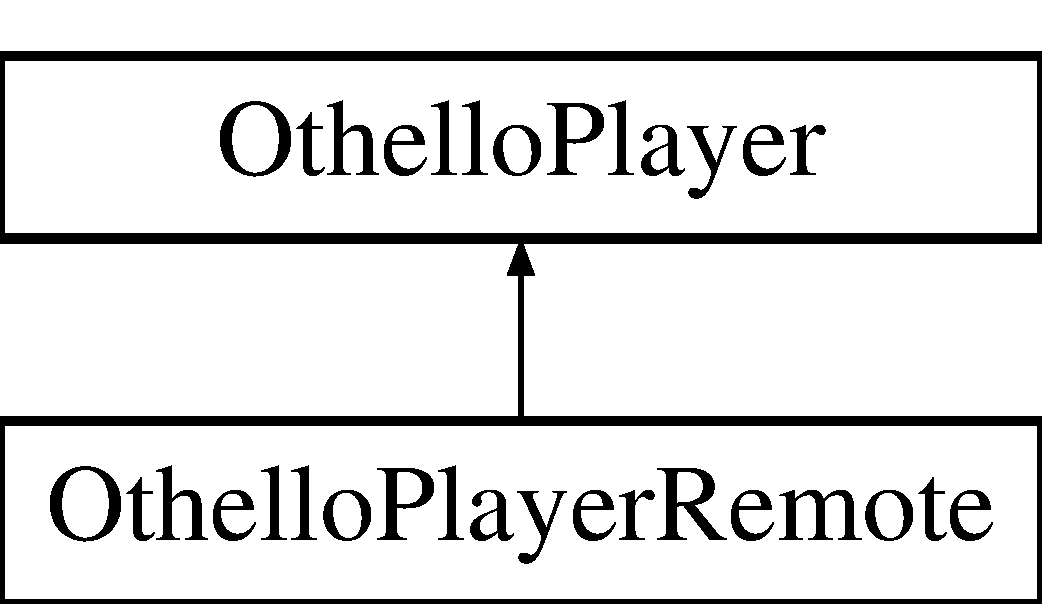
\includegraphics[height=2.000000cm]{classOthelloPlayerRemote}
\end{center}
\end{figure}
\subsection*{Public Member Functions}
\begin{DoxyCompactItemize}
\item 
\hypertarget{classOthelloPlayerRemote_ae06abf8567284ffdefe13da89fe99138}{{\bfseries Othello\-Player\-Remote} (int sockd)}\label{classOthelloPlayerRemote_ae06abf8567284ffdefe13da89fe99138}

\item 
void \hyperlink{classOthelloPlayerRemote_a6d7f6c0544aa6a6eb219e69d6c6d2e41}{winner} (const unsigned char winner, const \hyperlink{classOthelloBoard}{Othello\-Board}$<$ 8, 8 $>$ \&board)
\end{DoxyCompactItemize}
\subsection*{Additional Inherited Members}


\subsection{Member Function Documentation}
\hypertarget{classOthelloPlayerRemote_a6d7f6c0544aa6a6eb219e69d6c6d2e41}{\index{Othello\-Player\-Remote@{Othello\-Player\-Remote}!winner@{winner}}
\index{winner@{winner}!OthelloPlayerRemote@{Othello\-Player\-Remote}}
\subsubsection[{winner}]{\setlength{\rightskip}{0pt plus 5cm}void Othello\-Player\-Remote\-::winner (
\begin{DoxyParamCaption}
\item[{const unsigned char}]{winner, }
\item[{const {\bf Othello\-Board}$<$ 8, 8 $>$ \&}]{board}
\end{DoxyParamCaption}
)\hspace{0.3cm}{\ttfamily [inline]}, {\ttfamily [virtual]}}}\label{classOthelloPlayerRemote_a6d7f6c0544aa6a6eb219e69d6c6d2e41}
This function is used to inform the \hyperlink{classOthelloPlayer}{Othello\-Player} which of the players won the game and provide the final board state. It is optional to redefine this method. The player may choose to ignore this information, in which case the default definition is sufficient. 
\begin{DoxyParams}{Parameters}
{\em winner} & The player position of the winning player \\
\hline
{\em The} & board state at the end of the game \\
\hline
\end{DoxyParams}


Reimplemented from \hyperlink{classOthelloPlayer_a278b0f93b676c302f914a3dac85d5adf}{Othello\-Player}.



The documentation for this class was generated from the following file\-:\begin{DoxyCompactItemize}
\item 
/home/travis/build/pastika/\-Othello/othello\-Player\-Remote.\-h\end{DoxyCompactItemize}

\hypertarget{classOthelloPlayerTelnet}{\section{Othello\-Player\-Telnet Class Reference}
\label{classOthelloPlayerTelnet}\index{Othello\-Player\-Telnet@{Othello\-Player\-Telnet}}
}
Inheritance diagram for Othello\-Player\-Telnet\-:\begin{figure}[H]
\begin{center}
\leavevmode
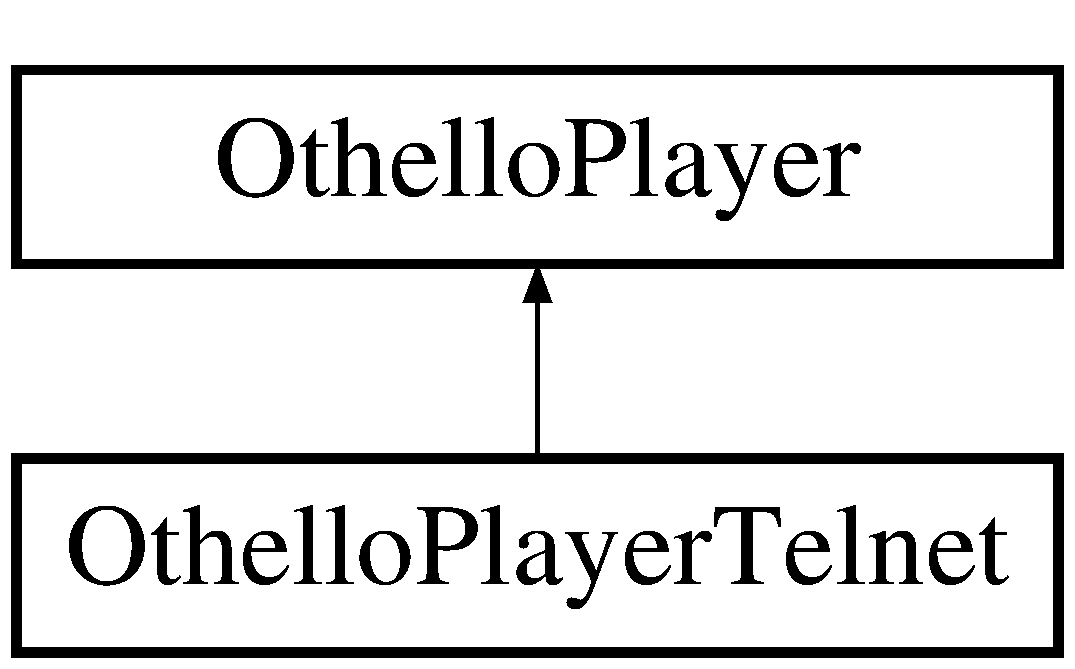
\includegraphics[height=2.000000cm]{classOthelloPlayerTelnet}
\end{center}
\end{figure}
\subsection*{Public Member Functions}
\begin{DoxyCompactItemize}
\item 
\hypertarget{classOthelloPlayerTelnet_a6d5600e72342f5bf6ce0c5e9300403a0}{{\bfseries Othello\-Player\-Telnet} (int sockd)}\label{classOthelloPlayerTelnet_a6d5600e72342f5bf6ce0c5e9300403a0}

\item 
void \hyperlink{classOthelloPlayerTelnet_a2903532fbbc2de163b4bf3c14e214dfe}{winner} (const unsigned char winner, const \hyperlink{classOthelloBoard}{Othello\-Board}$<$ 8, 8 $>$ \&board)
\end{DoxyCompactItemize}
\subsection*{Additional Inherited Members}


\subsection{Member Function Documentation}
\hypertarget{classOthelloPlayerTelnet_a2903532fbbc2de163b4bf3c14e214dfe}{\index{Othello\-Player\-Telnet@{Othello\-Player\-Telnet}!winner@{winner}}
\index{winner@{winner}!OthelloPlayerTelnet@{Othello\-Player\-Telnet}}
\subsubsection[{winner}]{\setlength{\rightskip}{0pt plus 5cm}void Othello\-Player\-Telnet\-::winner (
\begin{DoxyParamCaption}
\item[{const unsigned char}]{winner, }
\item[{const {\bf Othello\-Board}$<$ 8, 8 $>$ \&}]{board}
\end{DoxyParamCaption}
)\hspace{0.3cm}{\ttfamily [inline]}, {\ttfamily [virtual]}}}\label{classOthelloPlayerTelnet_a2903532fbbc2de163b4bf3c14e214dfe}
This function is used to inform the \hyperlink{classOthelloPlayer}{Othello\-Player} which of the players won the game and provide the final board state. It is optional to redefine this method. The player may choose to ignore this information, in which case the default definition is sufficient. 
\begin{DoxyParams}{Parameters}
{\em winner} & The player position of the winning player \\
\hline
{\em The} & board state at the end of the game \\
\hline
\end{DoxyParams}


Reimplemented from \hyperlink{classOthelloPlayer_a278b0f93b676c302f914a3dac85d5adf}{Othello\-Player}.



The documentation for this class was generated from the following file\-:\begin{DoxyCompactItemize}
\item 
/home/travis/build/pastika/\-Othello/othello\-Player\-Telnet.\-h\end{DoxyCompactItemize}

%--- End generated contents ---

% Index
\newpage
\phantomsection
\addcontentsline{toc}{chapter}{Index}
\printindex

\end{document}
